
\section{Implementation of the Artifact}

This section will describe the iterative process of implementing the larger artifact and is broken up into 3 subsections.
While these steps where happening concurrently, they each address a different aspect of the project and therefore underwent their own iterative processes.



\subsection{Infrastructure}


\subsubsection{First iteration - Minikube}
As the decision of the Workflow management tool was made, it was obvious that a dedicated \ac{k8s} infrastructure was needed to run the tool\footcite{PachydermDocsOnPrem}.
The Pachyderm documentation gave two recommendations for setting up an initial development environment, preferably Docker Desktop or alternatively Minikube \footcite{PachydermDocsLocal}.
Due to the exclusive license of Docker-Desktop\footcite{DockerTermsService2022},
which prevents large companies free usage of the product\footcite{DockerFAQsDocker2021} the choice fell on Minikube for an initial test setup.

In addition to the underlying \ac{k8s} Pachyderm also needs an external S3 Storage Bucket for its \ac{PFS} for which we used MinIO,
a self hostable S3 compliant object storage\footcite{incMinIOMinIOKubernetes}, which was also based on recommendations by the Pachyderm documentation.

The persistent storage requirements for the Pachyderm itself was fulfilled by manually creating two \ac{PV}'s on the hosts local harddrive.
Using the Helm packagemanager\footcite{HelmDocsHome} for \ac{k8s} the at that point newest version 2.6.4 was installed from the official Artifacthub repository\footcite{ArtifacthubPachyderm}.

The hostsystem of this iteration was a single ProLiant DL385 Gen10 Plus running Ubuntu 22.04.3 LTS x86\_64.
During the setup every step was diligently noted and put into a repository\footcite{eckerthInstallationInstructionsMinikube}, alongside the needed scripts. 
The instructions can be found in the appendix at \ref{appendix:minikube_installation_instructions}.


\subsubsection*{Learnings from the first iteration}

The shortcomings of this naive first iteration became apparent very quickly, 
which was to be expected, as the goal of this iteration was to create a minimal working example to get a better understanding of the toolings and the underlying infrastructure.

The first and foremost issue where the limitations imposed by Minikubes reliance on an Internal \ac{VM},
during testing the inability to on the fly increase the resources of the \ac{VM} became a significant bottleneck.
At some point during the testing of \ref{tcp_hpc_workloads} the \ac{VM} was so overloaded that the installation was irreparably damaged which was seen as a sign to move on to the next iteration.

Another more subtle issue was the discrepancy between the experience a small scale \ac{k8s} installation within Minikube and a large scale \ac{k8s} cluster like the one that would be used in later steps of the project.
Therefore it was decided that a more realistic \ac{k8s} cluster would be needed for the next iteration, which became the Heydar cluster.

\subsubsection{Second iteration - Heydar Cluster}
\label{heydar_cluster}

Improving upon the shortcomings of the first iteration, the second iteration was based in the attempt to create a more realistic \ac{k8s} cluster.
To achieve this 20 ProLiant DL360 Gen9 Servers, running Ubuntu 22.04.3 LTS x86\_64 where used to create a bare metal \ac{k8s} cluster,
using kubeadm as it provides deep integration with the underlying infrastructure\footcite{CreatingClusterKubeadm}.

But a bare metal cluster also comes with its own set of challenges, as the cluster needs to be provisioned and configured manually.
In order to automate this process, the Ansible automation tool was used to set up all the nodes in praralel and to ensure that the all the nodes are in the same state.
Ansible is a declarative tool which allows for the automation of the provisioning and configuration of the cluster\footcite{Ansible2023}, by specifying the desired state of the cluster in a playbook and then applying it to the cluster.
The Ansible playbook used for the setup of the cluster can be found at \ref{appendix:ansible_setup_script}.

Which unknowingly caused conflict between the Ansible playbook and the maintenance scripts of the cluster as the Heydar machines.
As \ac{k8s} needs very specific configurations on the underlying infrastructure like the deactivation of swap space\footcite{InstallingKubeadm}.

This was resolved by consulting with the maintainer of the cluster and adjusting the Ansible playbook as well as the maintenance config for the cluster nodes accordingly, 
after we had identified the issue.


One important aspect of a production like cluster is the networking, as \ac{k8s} does not natively manage communication on a cluster level,
but instead relies on so called \ac{CNI}s to manage and abstract the underlying network infrastructure \footcite{ClusterNetworking}.

Here we where spoiled for choice once again, as there are a multitude of different \ac{CNI}s available, each with their own advantages and disadvantages.
The Kubernetes documentation provides a non exhaustive list of 17 different \ac{CNI}s\footcite{KubernetesCNIPlugins}, which all fulfill this essential task in different ways.
As the needs regarding the network plugin where not very specific at this point, the choice fell on Calico, as surface level research showed that it was a popular choice for bare metal clusters\footcite{ExploreNetworkPlugins},
provided security and enterprise support as well having a wide range of features\footcite{mehndirattaComparingKubernetesContainer}.
But Calico proved to be more difficult to setup than expected, after consulting with a college who set up a different cluster with Calico,
it was decided to use Flannel as a \ac{CNI} instead.
Flannel turned out to be much easier to setup and configure, as it is a very lightweight \ac{CNI} which is designed for bare metal clusters\footcite{Flannel2023}, 
and foregoes the more advanced security features of Calico. 

The Flannel configuration used for the cluster can be found at \ref{appendix:flannel_config} it is closely based on the example configuration provided by the Flannel documentation\footcite{FlannelInstallConfig}.

\subsubsection*{Learnings from the second iteration}

The second iteration was a significant improvement over the first iteration, as it provided a much more realistic environment for the development of the artifact.
But it also came with its own set of challenges, as the bare metal cluster needed to be provisioned and configured manually, which was a significant time investment.

What became apparent very quickly was that the solution for the provisioning of the \ac{PV} was no where near scalable,
as it relies on the local harddrive of the host machine and therefore must host the container on the same machine as the \ac{PV} which defeats the purpose of a multi node cluster in the first place.
Therefore a more scalable solution needs to be implemented for the next iteration.
A possible solution could be the use of distributed storage solutions like Ceph\footcite{CephIoHome} or GlusterFS\footcite{Gluster}  in combination with the Rook project \footcite{Rook}. 
which will need to be explored in future iterations.


As described in section XXX a service hosting \ac{FAM} will be needed in future iterations aswell.

\subsection{Tightly Coupled HPC Workloads} 
\label{tcp_hpc_workloads}

As described in section \ref{state_of_the_art_tcp} \ac{TCP} problems are a large part of the \ac{HPC} world,  but seem to lack native support in Pachyderm.
Pachyderm as it exists as of writing this thesis, is centralized around \ac{LCP} problems, as it is designed to work with large amounts of data but with each so called "datum" being independent of each other.
This is a very good fit for \ac{LCP} problems, and ties into their concepts of data lineage, versioning and providence.

\begin{figure}[htb]
    \centering
    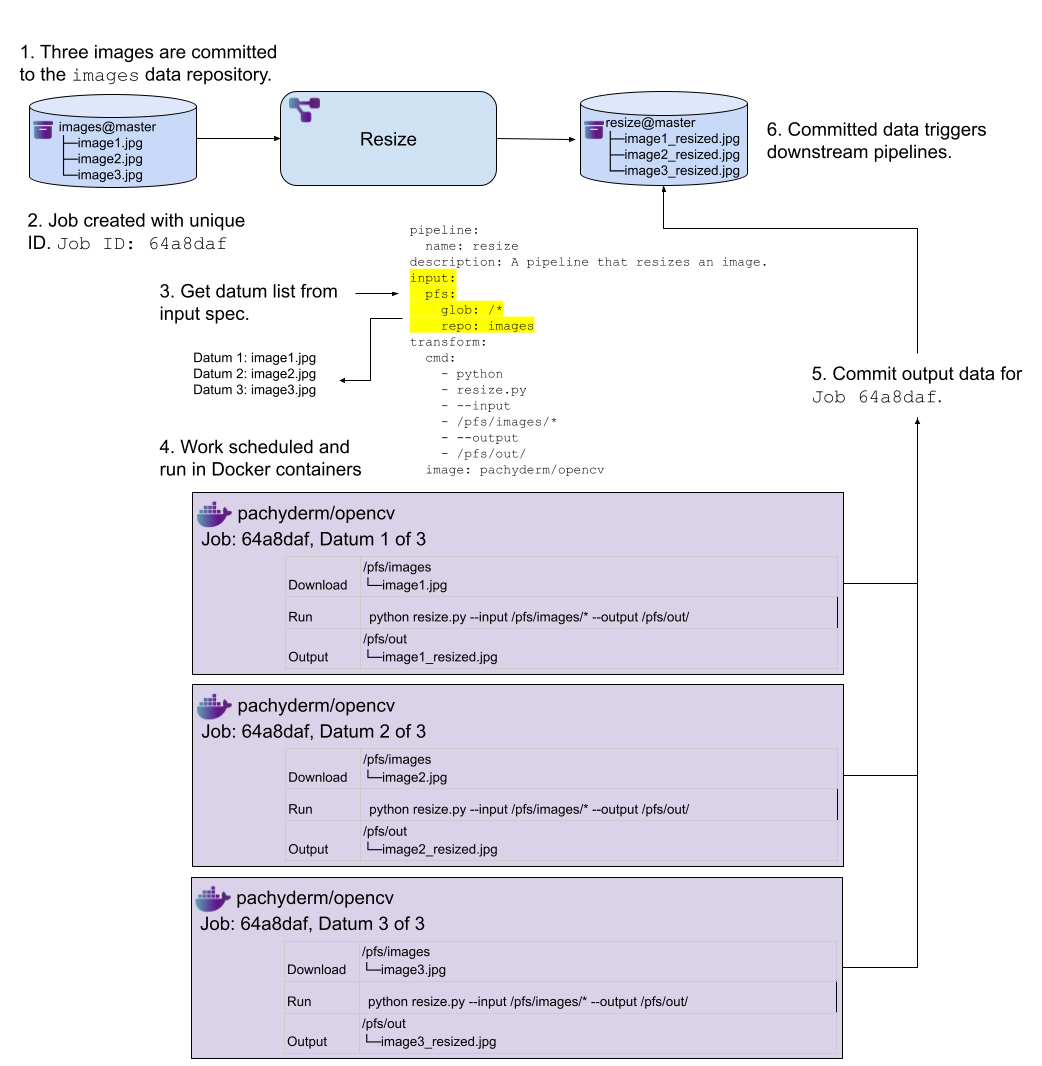
\includegraphics[width=14cm]{graphics/datum_distribution_amongst workers.png}
    \caption[Pachykouda datum distribution amongst workers]{Pachykouda datum distribution amongst workers \footnotemark}
    \label{abb:datum_distribution_amongst workers}
\end{figure}
\footnotetext{Taken from: \cite{IntroPipelines2023}}


Diagram \ref{abb:datum_distribution_amongst workers} shows Pachyderms approach to distribute their datums amongst workers, given an already defined pipeline.
Once Data files are added to the input repository, Pachyderm will determine Based on a glob pattern wether the files are relevant datums for the pipeline.
If the newly added data fits the pattern each of the files will be supplied to its own instantiation of a worker, all originating from the same image, which will then process the data concurrently and independently of each other.
After the worker has finished its task, the resulting datums are then collected in their own repository of data.
A more detailed swim lane diagram of this process can be found in the appendix at \ref{appendix:pipeline_communication_sld}.

This approach is very well suited for \ac{LCP} problems, as the datums are independent of each other and can be processed in parallel without any issues.
But it is not well suited for Large \ac{TCP} problems, if the computation of the data can not be split into distinct independent datum files, or the computation is reliant on the intercommunication of the datums.
If the datasets are small enough, this does not really present a problem as one can simply take all the data into a single workernode and process it there.
But as a single worker node can only utilize the resources of a single physical compute node, this does not scale well with the size of the dataset and defeats the purpose of a distributed system in the first place.

So our goal for this section is a way to find a way to enable pachyderm to pool the entire resources of the cluster, in oder to solve a \ac{TCP} problem.

\subsubsection{First iteration - PachyKouda}

As a first attempt to address this issue, it was decided that the integration of a \ac{TCP} framework into Pachyderm on the container level would be the best approach.
So the first iteration is based on the idea of a Pachyderm conforming client container, which is able to interface with an external \ac{TCP} framework,
which can handle the reception of the data, the distribution of the data amongst the workers and the collection of the results to reintegrate them into the \ac{PFS}.

The first iteration of this idea was called PachyKouda, as it was based on the Arkouda \ac{TCP} framework\footcite{ArkoudaGituhbRepository2023},
which itself is a python binding for the Chapel programming language \footcite{ChapellangChapelProductive}. 

For that step an Arkouda worker was installed bare metal on the headnode of the Heydar cluster, in order to verify the feasibility of the idea,
with the goal of moving the worker into the cluster in the next iteration.

The client container was based on the official \ac{UDP}-based build by the Arkouda team \footcite{ArkoudacontribArkoudadockerMain}.
The container was then modified to be able to communicate with the Arkouda worker on the headnode of the cluster, it can now send data to the worker and receive the results.

\subsubsection*{Learnings from the first iteration}

The first iteration was a total success, as it proved the feasibility of being able to use a client container to forward the data processing to an external Arkouda worker.
As described earlier, the goal of the next iteration is to move the Arkouda worker into the cluster, in order to be able to utilize the full resources of the cluster.

\subsubsection{Second iteration - Kymera}

\begin{figure}[htb]
    \centering
    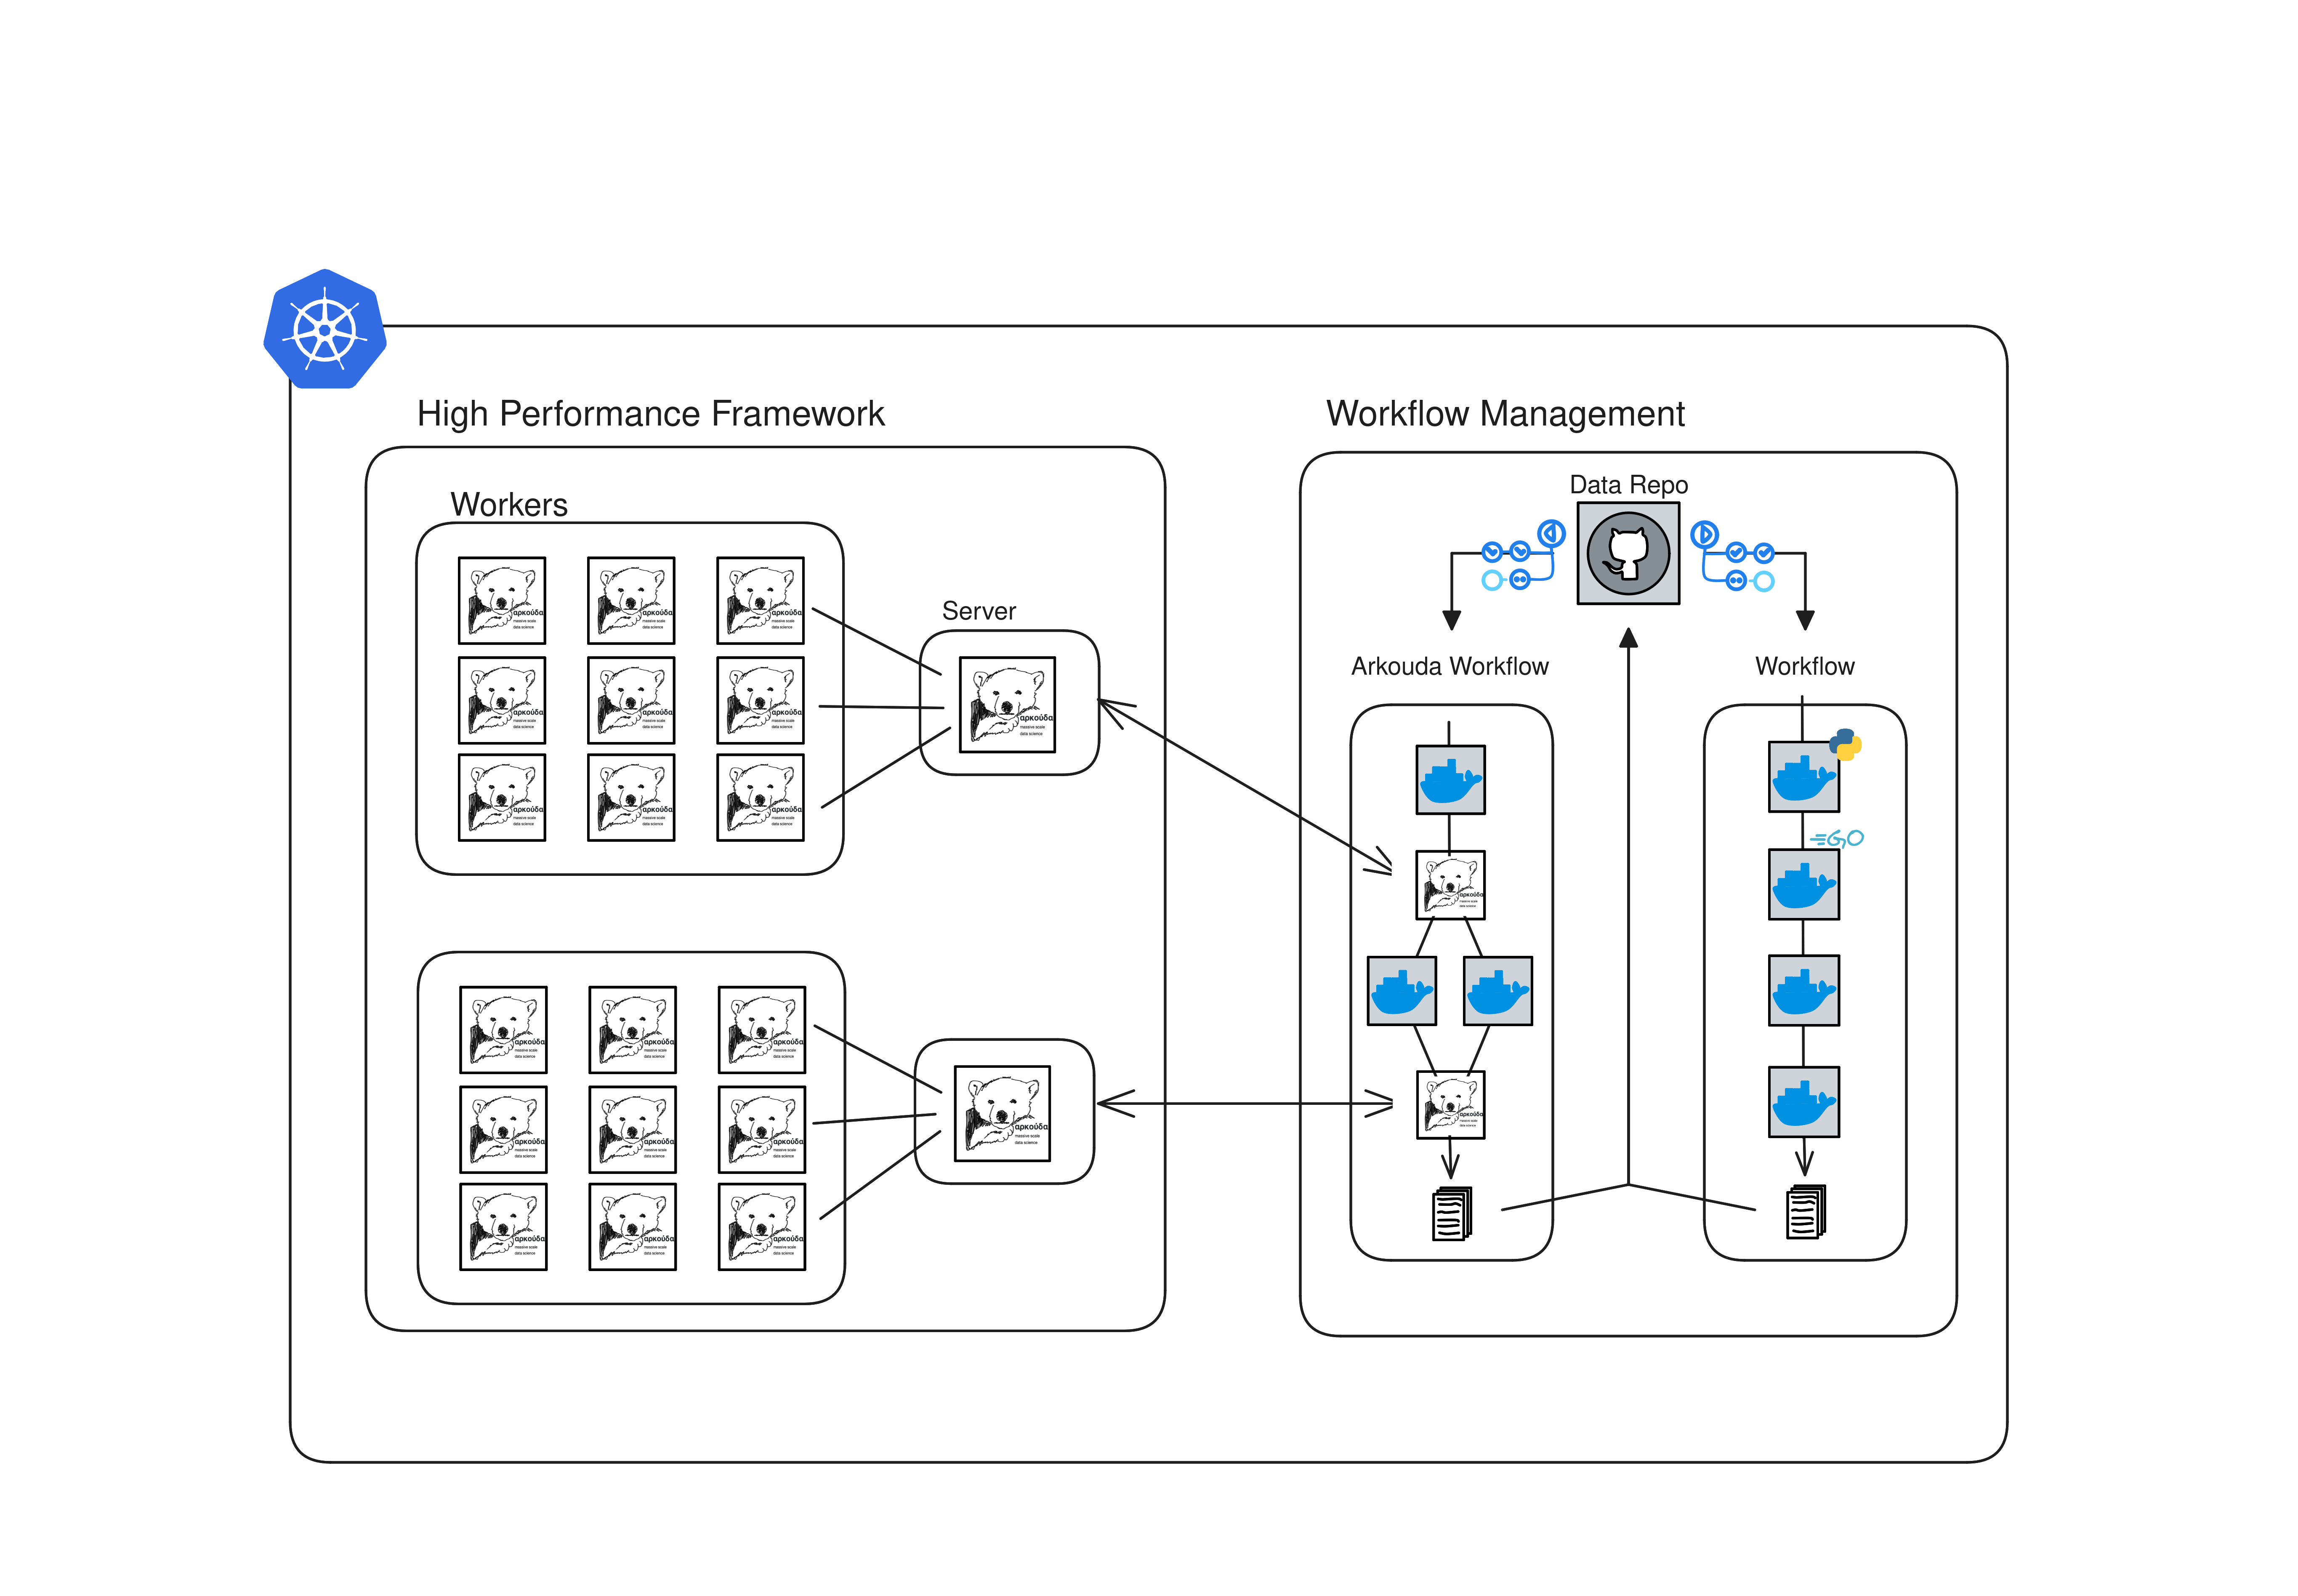
\includegraphics[width=16cm]{graphics/PachyKouda.png}
    \caption[Arkouda workers on \ac{k8s}]{Arkouda workers on the Heydar cluster}
    \label{abb:arkouda_workers_on_k8s}
\end{figure}

Diagram \ref{abb:arkouda_workers_on_k8s} above shows a high level overview of how the workers interface with the client container in the workflow.
The Arkouda container which is part of the workflow is still the same as in the first iteration, but now instead of interfacing with an external worker it 
is interfacing with a worker swarm hosted across the cluster.

The Swarm is split into two parts, one central Arkouda server, facilitating the communication between the client container and the workers and the workers also called locales themselves.
The locales and the server are based on the helm charts provided by the Arkouda-Contrip repo\footcite{BearsRUsArkoudacontribArkoudahelmcharts},

A detailed walk through the setup of the \ac{RBAC}, Secrets and deployments for the Heydar Cluster can be found in the appendix at \ref{appendix:arkouda_setup} which in turn is based on the official
Arkouda documentation\footcite{ArkoudacontribArkoudadockerMain}.

\subsubsection*{Learnings from the second iteration}
As Arkouda does not currently provide multi tenancy of their Server, meaning that they can only be connected a single client at a time, 
so if multiple pipelines need to solve a \ac{TCP} at the same time, they would not be able to share the same worker swarm.





\section*{Third iteration - \ac{FAM}}
% # THIS WIill be a table

% \begin{table}[htb]
    

% \subsubsection{Third iteration - \ac{FAM}} 

% \subsection{Supplementary Services}

% \subsubsection{Docker Registry}

% \subsubsection{Jenkins CI/CD Pipeline}

% \subsubsection{}


% \newpage    
